\textit{Anew}\cite{anew} es una herramienta escrita en \textit{Golang} que añade las líneas que salen por la salida estándar de un comando a un archivo concreto, pero solo si esas líneas no estaban ya contenidas en el archivo. También imprime en la salida estándar las nuevas líneas que se han añadido, funcionando de manera similar a como \texttt{tee -a} eliminando los duplicados.\\

Un ejemplo de su uso se muestra en la figura \ref{fig:anew-example}. En el ejemplo se tiene una lista inicial con el contenido ``\textit{uno}``, ``\textit{dos}`` y ``\textit{tres}``, y una segunda lista con más números: ``\textit{dos}``, ``\textit{tres}``, ``\textit{cuatro}`` y ``\textit{cinco}``. Ejecutando el comando \textit{anew} entre las dos listas, obtenemos como resultado los valores de la segunda lista que no están en la primera (``\textit{cuatro}`` y ``\textit{cinco}``), además de actualizar la primera lista con dichos valores.

\begin{figure}[h]
    \centering
    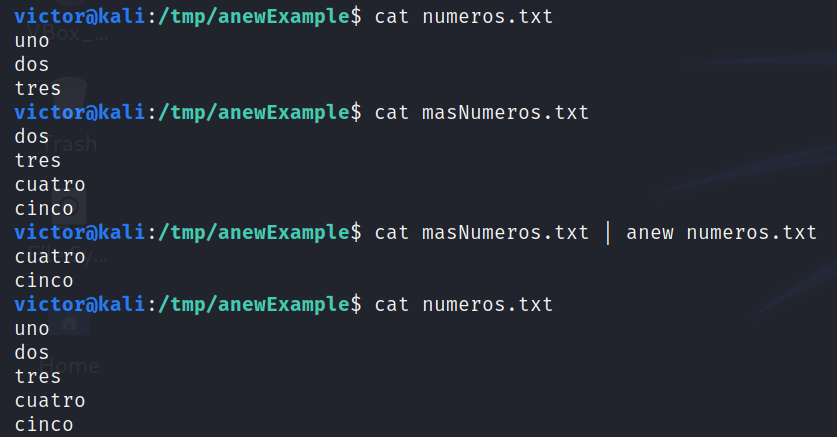
\includegraphics[width=0.60\textwidth]{images/sections/tools/anew-example.png}
    \caption{Ejemplo de uso de \textit{anew}}
    \label{fig:anew-example}
\end{figure}